\documentclass[11pt,border=5pt]{standalone}
\usepackage{fontspec}
\setmainfont{cmunrm.otf}[BoldFont=cmunbx.otf,ItalicFont=cmunti.otf,BoldItalicFont=cmunbi.otf]
\usepackage{amsmath}
\usepackage{unicode-math}
\setmathfont{NewCMMath-Regular.otf}
\usepackage{tikz}
\usetikzlibrary{arrows.meta,patterns,angles,quotes}
\begin{document}
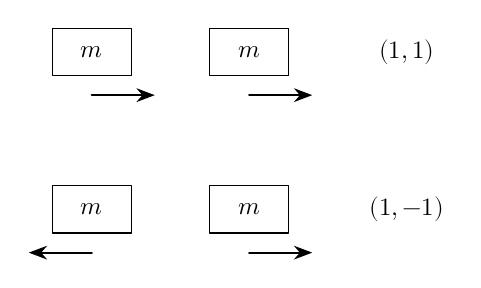
\begin{tikzpicture}[>=Stealth,font=\small,line cap=round,line join=round]
\draw[fill=white] (-1.5,0.7) rectangle (-0.5,1.3);
\node at (-1,1) {$m$};
\draw[fill=white] (0.5,0.7) rectangle (1.5,1.3);
\node at (1,1) {$m$};
\draw[->,thick] (-1,0.45) -- (-0.2,0.45);
\draw[->,thick] (1,0.45) -- (1.8,0.45);
\node at (3,1) {$(1,1)$};
\draw[fill=white] (-1.5,-1.3) rectangle (-0.5,-0.7);
\node at (-1,-1) {$m$};
\draw[fill=white] (0.5,-1.3) rectangle (1.5,-0.7);
\node at (1,-1) {$m$};
\draw[->,thick] (-1,-1.55) -- (-1.8,-1.55);
\draw[->,thick] (1,-1.55) -- (1.8,-1.55);
\node at (3,-1) {$(1,-1)$};

\end{tikzpicture}
\end{document}
